\chapter{LANGAGE HUMAIN ET COMMUNICATION ANIMALE}
\markright{Langage humain et communication animale}
\origpage{38}{024}
\begingroup\small\setstretch{1}\setlist[enumerate]{topsep=1pt,itemsep=1pt,parsep=0pt}\setlength{\parskip}{2pt}
\minititle{I.\quad HOMME ET ANIMAL : CONTINUITÉ OU DISCONTINUITÉ ?}
\begin{enumerate}[label=\arabic*.]
\item La thèse de la continuité
\begin{enumerate}[label=\textbf{\arabic*},nosep]
\item Gordon G. Gallup : test du miroir et conscience de soi
\item Jane Goodall : les outils chez chimpanzés
\item Les comportements sociaux et moraux
\end{enumerate}
\item La thèse de la discontinuité
\begin{enumerate}[label=\textbf{\arabic*},nosep]
\item Absence d’intentionnalité partagée
\item Absence de méta-outils
\item Absence de capacité syntaxique
\end{enumerate}
\end{enumerate}
\minititle{II.\quad MONTAIGNE : « IL N’EST DE MOUVEMENT QUI NE PARLE. »}
\begin{enumerate}[label=\arabic*.]
\item Montaigne : \textit{Apologie de Raymond Sebond}
\item Les signaux de la communication animale
\begin{enumerate}[label=\textbf{\arabic*},nosep]
\item Les signaux visuels
\item Les signaux vibratoires et acoustiques
\item Les signaux tactiles
\item Les signaux chimiques
\end{enumerate}
\item Communication verbale et non verbale
\begin{enumerate}[label=\textbf{\arabic*},nosep]
\item Le ratio d’Albert Mehrabian
\item Paul Ekman : la \textit{Basic Emotion Theory} (BET)
\end{enumerate}
\end{enumerate}
\minititle{III.\quad DESCARTES : « LES ANIMAUX SONT DES MACHINES. »}
\begin{enumerate}[label=\arabic*.]
\item Substance et étendue : le dualisme cartésien
\item La critique de Condillac : le \textit{Traité des animaux}
\end{enumerate}
\minititle{IV.\quad « LANGAGE » DES ABEILLES ET LANGAGE HUMAIN}
\begin{enumerate}[label=\arabic*.]
\item Karl Von Frisch : \textit{Vie et mœurs des abeilles}
\begin{enumerate}[label=\textbf{\arabic*},nosep]
\item L’expérience
\begin{enumerate}[label=\arabic*.]
\item La danse circulaire
\origpage{39}{025}
\item La danse en faucille
\item La danse frétillante
\end{enumerate}
\item Les premières conclusions
\begin{enumerate}[label=\arabic*.]
\item Points communs avec le langage humain
\item Les limites du « langage » animal
\end{enumerate}
\end{enumerate}
\item Émile Benveniste : caractéristiques du langage humain
\item Communication humaine et animale : tableau récapitulatif
\end{enumerate}
\minititle{Exercices}
\minititle{Pour aller plus loin}
\minititle{Glossaire}
\endgroup
\par\bigskip
\origpage{40}{026}
\lecturetitle{Introduction}
L’être humain est-il essentiellement un animal ou, au contraire, radicalement différent des autres espèces vivantes ? Dans le cas du langage, nous savons que les animaux communiquent entre eux, mais s’agit-il véritablement de langage ? Si ce n’est pas le cas, à partir de quel degré de complexité peut-on parler de langage ? Cette question a longtemps été le domaine réservé des philosophes. Dans ce chapitre, nous allons voir que pour Montaigne, il n’y a pas de différence de nature entre les deux, mais seulement de degré : c’est la thèse de la continuité. Les animaux, comme l’homme, parlent. Pour Descartes, au contraire, il existe une discontinuité radicale entre l’humain et l’animal, et seul l’homme possède un vrai langage. Comme souvent, la science moderne viendra nous éclairer, en particulier les travaux de Karl von Frisch sur la célèbre danse des abeilles. Sur la base de ces travaux, le linguiste français Émile Benveniste tracera une frontière nette entre langage humain et communication animale.
\section{HOMME ET ANIMAL : CONTINUITÉ OU DISCONTINUITÉ ?}
\markright{Homme et animal : continuité ou discontinuité ?}
\subsection{La thèse de la continuité}
Selon les partisans de la continuité, il n’existe pas de différence de nature entre l’homme et l’animal, et les caractéristiques que l’on avait longtemps crues spécifiques à l’humain ont aussi été constatées chez des animaux. Ces caractéristiques communes à l’homme et à l’animal sont comportementales (la bipédie), sociales (le tabou de l’inceste, la chasse, la guerre, la politique, la culture, le mensonge, la morale, l’empathie), et cognitives (la conscience de soi, l’utilisation d’outils, le langage, l’intelligence).
\subsubsection*{1\quad Gordon G. Gallup : test du miroir et conscience de soi}
Chez l’homme, c’est entre 12 et 18 mois que les enfants se reconnaissent dans un miroir. Ce « stade du miroir » a été découvert dans les années 30 par \textbf{Henri Wallon} (1879-1962), psychologue français et professeur au Collège de France. Le terme « stade du miroir » a ensuite été réutilisé par \textbf{Jacques Lacan} (1901-1981) en 1936 lors d’un congrès psychanalytique international à Marienbad puis en 1949 lors du 16\textsuperscript{e} congrès international de psychanalyse dans une communication intitulée : « Le stade du miroir comme formateur de la fonction du \textit{je} telle qu’elle nous est révélée dans l’expérience psychanalytique ». Ultérieurement, Lacan a développé un aspect important du stade du miroir en y introduisant une réflexion sur le rôle de \textit{l’autre} : selon lui, la fonction \textit{je} peut se mettre en place que par la présence de l’autre.\ednote{原文 « la fonction je peut se mettre en place que » 缺否定限制结构中的 ne，应为 « la fonction je ne peut se mettre en place que »。} Cela signifie que, pour les psychanalystes, dire « je » implique une opposition à l’autre.

La conscience de soi chez certains animaux a été révélée dans les années 1970 par le psychologue américain \textbf{Gordon G. Gallup} (1941-) au moyen du « test du miroir ». Appliqué aux animaux, ce test consiste à peindre un signe (une tache de couleur ou une croix) sur un animal à son insu \origcont{41}{027}(pendant son sommeil ou après anesthésie) puis à le placer face à un miroir. Au début, l’animal pense se trouver confronté à un congénère, mais certains individus présentent des comportements qui montrent qu’ils comprennent que le signe qu’ils voient dans le miroir se trouve sur leur propre corps. Gallup a constaté que des chimpanzés touchent la tâche avec leur main et que des éléphants touchent la croix avec leur trompe. Plus étonnant : une femelle dauphin se dirige vers le miroir. Voyant la tâche sur son corps, elle part alors frotter la partie de son corps marquée contre la paroi du bassin, puis faire plusieurs allers-retours entre le miroir et la paroi du bassin avec, à chaque fois, moins de substance colorée sur son corps : elle a identifié la tâche sur son corps, et essaie de l’enlever.\ednote{本段三处 « tâche » 均指身体上的色斑，应写作 « tache »，与前页的 « une tache de couleur » 一致。tâche 意为任务、工作。} Il est important de noter que seuls quelques rares animaux ont réussi le test du miroir : certains singes (bonobos, chimpanzés, orang-outans), dauphins, éléphants, corbeaux et perroquets.
\subsubsection*{2\quad Jane Goodall : les outils chez chimpanzés}
Dans les années 1960, l’anthropologue \textbf{Louis Leakey} (1903-1972) était convaincu que l’être humain était seul à utiliser des outils. Mais quelques années plus tard, celle qui avait son assistante,\ednote{原文 « celle qui avait son assistante » 不通，应为 « celle qui avait été son assistante »（曾担任其助手的人）。} \textbf{Jane Goodall} (1934-) a observé en octobre 1960 en Tanzanie un chimpanzé en train de fabriquer et d’utiliser des outils pour attraper des termites. Ses travaux ont profondément transformé les rapports homme-animal. Depuis, les observations de ce genre se sont multipliées : des chimpanzés introduisent une tige dans une fourmilière ou une termitière. Les insectes s’agrippent à la tige, les chimpanzés la retirent et mangent les insectes qui se trouvent sur la tige. Les primatologues ont révélé un autre comportement chez les chimpanzés : le cassage des noix. Les singes utilisent une pierre comme marteau et une grosse racine ou une pierre comme enclume. Bien d’autres usages d’outils ont également été constatés chez d’autres primates. Par exemple, on a récemment observé des gorilles utilisant des cannes pour mesurer la profondeur d’un cours d’eau, avant de le traverser.
\subsubsection*{3\quad Les comportements sociaux et moraux}
Si l’on sait depuis Aristote que l’homme est un animal social, on a quelque peu oublié que l’animal, est, si j’ose dire, un animal social. Les grands singes ont en effet des fonctionnements sociaux particulièrement complexes que l’on ne soupçonne guère. Ils peuvent par exemple faire usage de stratégies politiques : deux mâles peuvent se coaliser pour renverser le chef du groupe, et des chimpanzés peuvent servir de médiateurs lors de conflits. Les primatologues ont montré que les singes (surtout les bonobos) peuvent aussi manifester des sentiments d’empathie et de gratitude. Ils éprouvent le sentiment de ce qui est juste ou pas, peuvent faire preuve de générosité et d’altruisme. La découverte de ces comportements moraux et altruistes chez les animaux a bien sûr fortement bouleversé notre regard sur eux. L’empathie, en particulier, cette capacité à se mettre à la place des autres, a été observée chez des rats il y a déjà un demi-siècle. En 1959, un article du psychologue expérimental \textbf{Russell M. Church} au titre surprenant, « les réactions émotionnelles des rats à la douleur d’autrui », a montré que lors d’une expérience en laboratoire, les rats arrêtent d’appuyer sur un levier commandant la distribution de nourriture si cette action envoie en même temps une décharge électrique à un congénère. Bien avant Church, dès 1744, dans son ouvrage polémique \textit{L’Homme machine} (1744)\ednote{本句两次写 1744 有误。本次核对的 Leyde、Élie Luzac fils 版书名页标有 MDCCXLVIII，即 1748；引用该版应标 1748，而非 1744。初刊流通时间与书名页印年应区别处理。\ecite{11}}, le philosophe \textbf{Julien Offray de La Mettrie} (1709-1751) citait l’exemple d’animaux pris de remords ou capables de reconnaissance :
\origpage{42}{028}
\begin{lecture}{}
Le chien qui a mordu son maître qui l’agaçait, a paru s’en repentir le moment suivant ; on l’a vu triste, fâché, n’osant se montrer, s’avouer coupable par un air rampant et humilié. L’histoire nous offre un exemple célèbre d’un lion qui ne voulut pas déchirer un homme abandonné à sa fureur, parce qu’il le reconnut pour son Bienfaiteur.
\end{lecture}
On a vu jusqu’ici que ce qui semblait être à la fois l’apanage de l’homme et les conditions de l’apparition du langage, à savoir la vie en société, l’utilisation d’outils et la conscience de soi, sont observés chez certains animaux.
\subsection{La thèse de la discontinuité}
Les partisans de la thèse de la discontinuité entre l’animal et l’être humain reconnaissent que les animaux (surtout les grands singes) ont des aptitudes bien supérieures à ce que l’on croyait initialement, qui n’atteignent pas le même niveau de complexité que chez l’être humain. En fait, l’impression générale qui ressort de leurs travaux est que l’être humain est le seul à atteindre un niveau « méta », c’est-à-dire de second degré, dans beaucoup d’opérations, et en particulier les opérations cognitives.
\subsubsection*{1\quad Absence d’intentionnalité partagée}
Le psychologue cognitif américain \textbf{Michael Tomasello} (1950-) est l’un des plus fervents partisans de la thèse de la discontinuité. Il affirme que, certes, l’être humain partage certaines caractéristiques avec les grands singes, mais que la cognition humaine est unique en raison de sa nature collective. En 2005, Tomasello a publié un article expliquant que la différence cruciale entre la cognition humaine et celles des autres espèces est l’« intentionnalité partagée », c’est-à-dire l’aptitude à participer avec les autres à des activités en collaboration, sur la base d’intentions et d’objectifs communs. Pour Tomasello, même si certains animaux peuvent comprendre les objectifs et intentions des autres, seul l’être humain possède la motivation de partager ces éléments pour agir avec d’autres. Plusieurs spécialistes de la question ont écrit des commentaires critiques sur cet article, affirmant que les tactiques de chasse des chimpanzés, des lions et des hyènes par exemple, sont fondées sur une « intentionnalité partagée ». Mais Tomasello leur a répondu que la chasse en commun peut très bien être le résultat de l’addition d’actions individuelles plutôt que le fruit d’une intention partagée.
\subsubsection*{2\quad Absence de méta-outils}
Autre argument des partisans de la thèse de la discontinuité : bien que certaines espèces utilisent des outils, il ne semble pas qu’elles utilisent des méta-outils, c’est-à-dire des outils destinés à fabriquer d’autres outils. Mais tout dépend du sens que l’on donne aux mots. En effet, pour certains chercheurs, les chimpanzés utilisent un méta-outil lorsqu’ils se servent d’un caillou pour stabiliser l’enclume de pierre qui leur sert à casser des noix. Parce que le débat persiste sur la définition de l’outil, le psychologue spécialiste de la cognition animale \textbf{Benjamin B. Beck} a édicté dans \textit{Animal tool behavior : the use and manufacture of tools by animals} (1980) les trois conditions qui satisfont \origcont{43}{029}à la définition d’un « outil » chez l’animal:
\begin{itemize}
\item L’objet doit être détaché de son substrat et se trouver à l’extérieur du corps de l’utilisateur.
\item L’utilisateur de l’outil doit le tenir ou le porter au moment de son usage ou juste avant et il doit l’orienter correctement par rapport au but.
\item La mise en œuvre d’un outil doit comporter un changement dans la forme, dans la position ou dans la condition d’un autre objet, d’un autre organisme ou de l’utilisateur lui-même.
\end{itemize}
\subsubsection*{3\quad Absence de capacité syntaxique}
Grâce à la langue des signes, certains chimpanzés sont parvenus à apprendre plusieurs centaines de mots, voire mille dans le cas du bonobo Kanzi.\ednote{此处把 Kanzi 的语言研究笼统归入“手语”不准确。有关研究涉及英语口语理解和 lexigram 图形符号系统；研究机构也明确说明它用图形符号键盘表达请求。词汇量还须区别听懂口语、识认符号与主动使用，不宜把本句的“千词”径直理解为掌握千个手语词。\ecite{8}} Pour le primatologue américain, \textbf{David Premack} (1925-2015), qui a enseigné la langue des signes à Sarah, une femelle chimpanzé, les grands singes sont certes intelligents et capables d’abstraction, mais leur capacité à utiliser un langage est très limitée. La capacité syntaxique, c’est-à-dire l’aptitude à combiner des mots simples pour former de nouvelles significations, leur est quasiment étrangère. Selon le professeur de psychologie cognitive \textbf{Jacques Vauclair} (1947-), cette capacité chez les primates ne dépasse pas le stade d’une grammaire à deux mots. Quant aux compétences langagières de Kanzi, malgré ses mille mots, elles ont stagné et ne dépasseront jamais le niveau d’un enfant de 3 à 4 ans.\ednote{本段“永远不会超过三至四岁儿童”的表述强于其所给证据。具体任务的成绩不能直接确定所有语言能力的永久年龄上限；1993 年对 Kanzi 和一名儿童的研究报告了对新句子及某些简单句法手段的理解。这也不等于两者具有完全相同的语言能力。\ecite{8}}

Entre la thèse de la continuité et celle de la discontinuité, Montaigne se situe résolument dans la continuité, et il ne fait aucun doute pour lui que les animaux « parlent ».
\section{MONTAIGNE : « IL N’EST DE MOUVEMENT QUI NE PARLE. »}
\markright{Montaigne : mouvements et communication}
Dans le premier chapitre, nous avons vu que Dieu a créé l’homme afin que ce dernier domine les animaux. Dans son \textit{Apologie de Raimond Sebond}, Montaigne va s’opposer avec force à cette idée. Pour lui, l’homme se situe au même niveau que l’animal.
\subsection{Montaigne : \textit{Apologie de Raymond Sebond}}
L’idée de la domination de la nature par l’homme a été reprise au 15\textsuperscript{e} siècle par le philosophe humaniste catalan Raymond Sebond (1385-1436). Dans sa \textit{Théologie naturelle} (1436), il voit en l’homme le souverain de la création. Entre 1568 et 1569, à la demande de son père, Montaigne va traduire l’ouvrage de Sebond (qui écrivait en latin) et intégrer à ses \textit{Essais} une longue apologie de son auteur. Mais cet éloge va tourner à l’éloge paradoxal : Montaigne va y accumuler les exemples évidents de la supériorité morale de l’animal et de l’insuffisance de la raison humaine.
\origpage{44}{030}
\begin{lecture}{Lecture : \textit{Apologie de Raymond Sebond} (extrait)}
La presomption est nostre maladie naturelle et originelle. La plus calamiteuse et fragile de toutes les creatures c’est l’homme, et quant et quant, la plus orgueilleuse. [...] C’est par la vanité de ceste mesme imagination qu’il s’égale à Dieu, qu’il s’attribue les conditions divines, qu’il se trie soy-mesme et separe de la presse des autres creatures, taille les parts aux animaux ses confreres et compagnons, et leur distribue telle portion de facultez et de forces, que bon luy semble. Comment cognoist il par l’effort de son intelligence, les branles internes et secrets des animaux ? Par quelle comparaison d’eux à nous conclud il la bestise qu’il leur attribue ? Au demeurant nous decouvrons bien evidemment, qu’entre elles il y a une pleine et entiere communication, et qu’elles s’entendent, non seulement celles de mesme espece, mais aussi d’espèces diverses. En certain abboyer du chien, le cheval cognoist qu’il y a de la colere : de certaine autre sienne voix, il ne s’effraye point. Aux bestes mesmes qui n’ont pas de voix, par la societé d’offices, que nous voyons entre elles, nous argumentons aisément quelque autre moyen de communication : leurs mouvemens discourent et traictent.
\begin{center}
Etmutæ pecudes, Et denique secla ferarum\\
Dissimiles suerunt voces variásque cluere\\
Cum metus aut dolor est, aut cum jam gaudia gliscunt
\end{center}
Et les bêtes privées de la parole et même les animaux sauvages font entendre des cris différents et variés, selon que la crainte, la douleur ou la joie les agite. (Lucrèce, V, 1058)
\begin{center}
Nonalia longè ratione atque ipsa videtur\\
Protrahere ad gestum pueros infantia linguæ
\end{center}
C’est à peu près de la même manière qu’on voit les enfants conduits au langage des gestes par l’impuissance de leur langue.

Pourquoy non, tout aussi bien que nos muets disputent, argumentent, et content des histoires par signes ? J’en ay veu de si souples et formez à cela, qu’à la verité, il ne leur manquoit rien à la perfection de se savoir faire entendre. Les amoureux se courroussent, se reconcilient, se prient, se remercient, s’assignent, et disent en fin toutes choses des yeux.
\begin{center}
E’l silentio ancor suole\\
Haver prieghi e parole
\end{center}
Le silence même sait prier et se faire entendre. (Le Tasse, Aminta, II)

[...] Quoy des sourcils ? Quoy des espaules ? Il n’est mouvement, qui ne parle, et un langage intelligible sans discipline, et un langage publique. Qui fait, voyant la varieté et usage distingué des autres, que cestuy-cy doibt plustost estre jugé le propre de l’humaine nature. Je laisse à part ce que particulierement la necessité en apprend soudain à ceux qui en ont besoing ; et les alphabets des doigts, et grammaires en gestes ; et les sciences qui ne s’exercent et ne s’expriment que par iceux.
\end{lecture}
\origpage{45}{031}
\begin{itemize}
\item Dans cet extrait, Montaigne réfute toute idée de supériorité de l’homme sur l’animal. C’est en effet par présomption, prétention, vanité que l’homme se croit au dessus de l’animal, et c’est sa maladie « originelle ».
\item Montaigne note que les animaux qui n’ont pas de « voix », c’est-à-dire qui ne communiquent pas au moyen de signaux sonores, disposent « de quelque autre moyen » : ce moyen, ce sont leurs mouvements, qui « discourent et traictent ». On comprend que pour Montaigne, les animaux parlent (« discourent ») avec leur corps. Or, le verbe « discourir » employé par Montaigne vient du grec \textit{logos} qui, on le sait, signifie aussi « langage ».\ednote{这里混淆了意义关联与词源。discourir 的词源属拉丁语 discurrere 一系，并非希腊语 logos；不能由 logos 的多义性推出法语 discourir 的词源关系。\ecite{12}} Si les animaux « discourent », alors, il existe bien un langage animal.
\item Pour appuyer son argumentation, Montaigne cite Lucrèce, poète latin du 1er siècle avant J.-C. et auteur du très célèbre poème \textit{De natura rerum} (« De la nature »). Les animaux, dit Lucrèce, savent avec leur cris exprimer « crainte », « douleur » et « joie ». On retrouve ici très exactement l’idée de « voix » expressive vue chez Aristote dans le chapitre précédent : « la voix ne sert qu’à indiquer la joie et la peine, et appartient aux animaux également (car leur nature va jusqu’à éprouver les sensations de plaisir et de douleur, et à se les signifier les uns aux autres). »
\item « L’impuissance de la langue » chez les enfants qui amène au « langage des gestes » permet à Montaigne de quitter temporairement les animaux et pour passer à l’homme, et plus précisément aux muets privés de parole.
\item Avec les mouvements de leur corps, au moyen d’une langue qui ne parle qu’aux yeux, les muets peuvent tout exprimer : « nos muets disputent, argumentent, et content des histoires par signes ? J’en ay veu de si souples et formez à cela, qu’à la verité, il ne leur manquoit rien à la perfection de se savoir faire entendre. » Cette idée est importante, car selon Montaigne, la langue des signes a la même « perfection » que la langue des hommes dotés de la parole. Pour cette notion de « perfection », nous la retrouverons tout à l’heure dans un texte de Descartes, où il la retournera contre Montaigne pour le réfuter.
\item La conclusion qu’il en tire est claire : « Il n’est mouvement qui ne parle. » Pour Montaigne le corps tout entier « signifie ». C’est un langage corporel inné (« sans discipline »), constitué d’un « alphabet des doigts » et « une grammaire des gestes ». Voilà qui est joliment dit.
\item S’il peut ainsi soutenir la thèse d’un langage animal, c’est parce qu’il nie la primauté et la spécificité du langage verbal par rapport à la communication gestuelle des muets et des animaux.
\end{itemize}
L’erreur de Montaigne, si l’on peut dire, vient d’un usage inadapté du verbe « parler ». De nos jours, on dira (et tout le monde admet) que les animaux ne « parlent » pas mais « communiquent ». Néanmoins, il est remarquable de noter que les sciences de la communication modernes ont validé le point de vue de Montaigne sur l’existence d’une communication « sans voix », c’est-à-dire non verbale.
\origpage{46}{032}
\subsection{Les signaux de la communication animale}
L’éthologie est la science qui étudie le comportement des animaux dans leur milieu naturel. Elle définit la communication animale comme un « processus par lequel un individu émetteur influence le comportement d’un autre individu, le récepteur, en lui adressant des signaux ». Ce qu’Aristote ou Montaigne appellent « voix » est en fait un signal sonore. Mais la communication animale présente une extrême diversité dans ses manifestations et donc plusieurs types de signaux sont utilisés simultanément par les animaux. Quand Montaigne écrivait plus haut « aux bestes mesmes qui n’ont pas de voix [...] nous argumentons aisément quelque autre moyen de communication », il avait raison. L’éthologie a monté que quatre types de signaux sont fréquemment utilisé par les animaux.\ednote{原文 « a monté »、« sont fréquemment utilisé » 应分别为 « a montré »、« sont fréquemment utilisés »。}
\subsubsection*{1\quad Les signaux visuels}
Les gestes sont la méthode de communication la plus connue, utilisée par diverses espèces, dont l’ensemble des primates. Comme chez l’homme, l’expression faciale permet de deviner certaines émotions d’un animal afin d’agir et réagir en conséquence. Ainsi, on saura par exemple qu’un chien est en colère lorsqu’il montre ses dents ou heureux lorsqu’il remue la queue. Les exemples dans la nature sont extrêmement nombreux, allant du changement de couleur chez le caméléon. En revanche, l’inconvénient majeur de la communication visuelle est son dépendance à la présence d’une source extérieure de lumière.\ednote{原文 « son dépendance » 中 dépendance 为阴性，应为 « sa dépendance »。} La nuit (ou à partir de dix mètres sous la surface des océans), les signaux visuels deviennent inutilisables, sauf si les animaux possèdent un moyen de produire de la lumière, comme les lucioles.\ednote{“海面下十米起视觉信号便无法使用”有误。海水透光随水质等条件变化；NOAA 的说明将通常有显著日光的表层范围概括为约二百米，适当条件下更深处仍能检出微弱日光。不能把十米当作统一的无光界限。夜间是否能使用视觉信号也取决于环境光和视觉适应。\ecite{9}}
\subsubsection*{2\quad Les signaux vibratoires et acoustiques}
La communication vocale à travers des signaux acoustiques concerne aussi de très nombreuses espèces telles que les oiseaux, mais aussi les baleines, les singes ou encore les chiens, qui utilisent des signaux sonores extrêmement variés leur permettant de décrire à leurs congénères le type, la taille et même la vitesse d’un prédateur. Puisque physiquement le son est une onde vibratoire, on considère que les signaux sonores forment un sous-ensemble de la famille des signaux vibratoires. Les éléphants émettent de tels signaux vibratoires en frappant le sol de leurs pattes, et des congénères se trouvant à plusieurs kilomètres de distance sont capables de percevoir la vibration du sol et interpréter ce signal.
\subsubsection*{3\quad Les signaux tactiles}
Le toucher peut aussi être un facteur important lors des interactions sociales, des combats ou de la reproduction, mais il n’est pas sans inconvénients : ce mode de communication ne peut être mis en œuvre que lorsque les protagonistes sont très proches l’un de l’autre. La portée des signaux tactiles est très limitée. En revanche, à la différence des signaux visuels, ils ne dépendent pas de la présence de lumière.
\subsubsection*{4\quad Les signaux chimiques}
L’utilisation de signaux chimiques constitue la méthode de communication la plus ancienne. Dès l’apparition des premiers êtres vivants (bactéries) jusqu’à celle des êtres les plus organisés \origcont{47}{033}(mammifères, insectes, etc.), la communication chimique sous forme d’échange de molécules, a en effet été le système de communication le plus universellement utilisé. La communication chimique, essentielle dans la reproduction pour de nombreuses espèces, intervient aussi dans les liens sociaux à travers la notion de « signature chimique ». On peut bien sûr penser aux fourmis, mais les insectes ne sonts pas les seuls à communiquer chimiquement :\ednote{原文 « ne sonts pas » 应为 « ne sont pas »。} les mammifères en sont aussi capables et utilisent des signaux chimiques pour marquer leur territoire.

Montaigne, adepte de la thèse de la continuité entre l’homme et l’animal a trouvé au 17\textsuperscript{e} siècle un contradicteur de poids en la personne de René Descartes.
\subsection{Communication verbale et non verbale}
L’anthropologue, psychologue, et épistémologue américain \textbf{Gregory Bateson} (1904-1990)\ednote{卒年误为 1990，应为 1980；Gregory Bateson 生卒年为 1904—1980。\ecite{10}} a fondé en Californie dans les années 50 la très célèbre École de Palo Alto, renommée dans le monde entier pour ses recherches en psychologie, psycho-sociologie, sciences de l’information et cybernétique. Selon Bateson, « on ne peut pas ne pas communiquer ». On peut cesser de parler, mais notre corps, lui, ne cessera pas de « signifier » malgré nous. Pour lui, tout comportement est communication. Toute conversation, tout échange, n’a pas forcément recours à la parole. La communication repose sur les mots, mais aussi sur les gestes, les attitudes, et les expressions faciales. Dans cette optique, le corps « parle » et transmet des messages aussi efficaces que les mots que l’on prononce. De plus, nos interlocuteurs réagissent inconsciemment à nos messages et ne se rendent pas compte qu’ils nous communiquent à leur tour de nombreuses informations à leur insu. On peut alors se demander quelle est la part respective de la communication verbale et non verbale dans notre vie quotidienne. La réponse ci-dessous ne manquera pas de vous étonner.
\subsubsection*{1\quad Le ratio d’Albert Mehrabian}
Bien avant Montaigne, on avait déjà perçu dès l’antiquité l’importance de la communication non verbale. Ainsi, dans la tradition gréco-romaine, les orateurs étaient conscients de la nécessité d’utiliser les expressions faciales, les mains, mais aussi les intonations de la voix pour donner de la force à leur discours. La grand orateur romain \textbf{Cicéron} (106-43 avant J.-C.),\ednote{原文 « La grand orateur » 应为 « Le grand orateur »。} a écrit dans un de ses traités de rhétorique que « les gestes sont l’éloquence du corps ». Tous les traités de rhétorique de l’époque insistent sur le rapport indissociable entre parole et geste. À l’époque moderne, la communication non verbale a fait l’objet de très nombreuses recherches. La plus connue est celle d’\textbf{Albert Mehrabian} (1939-), psychologue et professeur à l’Université de Californie. En 1967, il a formulé la « règle du 7\% -38\% -55\% », appelée aussi « règle des 3V ». Selon cette règle :
\begin{itemize}
\item 7\% de la communication est verbale, et passe par la signification des mots.
\item 38\% de la communication est vocale, et se transmet par les intonations et les sons de la voix.
\item 55\% de la communication est visuelle, basée sur les expressions du visage et sur le langage corporel.
\end{itemize}
Ce ratio d’Albert Mehrabian permet de relativiser l’importance des mots, puisque 93\% de notre \origcont{48}{034}communication se passe d’eux.\ednote{本段把特定实验结果推广为一切交际的信息比例，错误。Mehrabian 本人的说明明确限定：这些比例来自情感和态度（喜欢／不喜欢）的传达实验，尤其涉及彼此不一致的线索；不能据此断言日常交际的 93\% 无需语言。公式的 55\% 指面部线索，亦不能无条件推广到全部身体动作。应更正为：在所研究的态度判断任务中，词语、声音和面部线索的相对权重约为 7、38、55；这些权重不是普遍的交际定律。\ecite{7}} Cette règle des 3V implique aussi que pour parler efficacement et significativement à autrui, il faut que les informations verbales, vocales et visuelles (les 3V) disent la même chose. Autrement dit, les mots que l’on utilise, notre intonation et les expressions de notre visage doivent en être en accord :\ednote{原文 « doivent en être en accord » 多出 en，应为 « doivent être en accord »。} c’est ce que Mehrabian appelle « congruence », que l’on peut rapprocher de la notion de concordance. Dans le cas contraire, notre interlocuteur pourra être troublé par des messages divergents et donc contradictoires.
\subsubsection*{2\quad Paul Ekman : la \textit{Basic Emotion Theory} (BET)}
Nous l’avons un peu plus haut :\ednote{原文 « Nous l’avons un peu plus haut » 缺过去分词，应为 « Nous l’avons vu un peu plus haut »。} pour le poète Lucrèce, « les bêtes privées de la parole » peuvent exprimer avec leur cris trois émotions : crainte, douleur et joie. Les travaux du psychologue américain \textbf{Paul Ekman} (1933-) ont permis de montrer que l’homme peut exprimer avec son visage sept émotions primaires (\textit{basic emotions}) déterminées non pas par la culture, mais par la biologie. Pour lui, ces expressions faciales sont universelles. Il rejoint ainsi l’opinion exprimée par Darwin dans son \textit{The expression of emotions in man and animals} (1872). En 1972, Ekman a dans un premier temps déterminé six émotions primaires universelles : la colère, le dégoût, la joie, la peur, la tristesse, et la surprise. Au début des années 1990, il a ajouté une 7ème émotion primaire universelle : le mépris. Ses travaux ultérieurs l’ont conduit à répertorier d’autres émotions plus difficiles à identifier sur le visage: les émotions secondaires, souvent produites par la combinaison de signaux appartenant aux émotions primaires. Ces émotions secondaires sont l’amusement, le plaisir des sens, le contentement, le soulagement, la fierté, l’embarras, la satisfaction, l’excitation, la haine, la culpabilité, et la honte. Au final, selon Ekman, ce sont en tout 16 émotions que notre visage peut exprimer sans utiliser le moindre mot.\ednote{本段内部计数不一致：前列七项“初级情绪”，后列十一项“次级情绪”，合计十八项，而非十六项。不能只把总数改成十八并当作 Ekman 的正式分类；原段把不同阶段、不同分类口径混合，具体“十六项”所据出处尚待核。} Ekman est aussi connu pour ses recherches sur les micro-expressions du visage, expressions dont la durée est comprise entre 1/15 et 1/20 de seconde. Très difficiles à feindre, elles sont utilisées de nos jours dans des programmes de détection du mensonge, car elles peuvent trahir l’absence de congruence entre les informations verbales, vocales et visuelles.
\clearpage
\section{DESCARTES : « LES ANIMAUX SONT DES MACHINES. »}
\markright{Descartes : les animaux sont des machines}
Pour \textbf{René Descartes} (1596-1650) les animaux sont assimilables à des machines sans pensée, et donc sans langage. La différence entre l’homme et l’animal n’est pas une différence de degré ou de complexité comme le pensait Aristote, mais une différence de nature. On pourrait dire, en utilisant la terminologie cartésienne, une différence de « substance ». Nous allons d’abord voir le « dualisme » de Descartes, avant d’analyser son argumentaire sur le silence des animaux.
\subsection{Substance et étendue : le dualisme cartésien}
Dans ses \textit{Méditations Métaphysiques} (1641), puis quelques années plus tard dans ses \textit{Principes de Philosophie} (1644), Descartes expose sa théorie du dualisme selon laquelle en l’homme coexistent deux types de substances. La première substance, appelée en latin \textit{res cogitans}, est la substance pensante, c’est-à-dire l’esprit. La seconde, \textit{res extensa} (« substance étendue »), est la substance corporelle, c’est-à-dire le corps. Comme, par définition, la substance mentale n’a pas d’étendue, et qu’inversement \origcont{49}{035}le corps ne peut pas penser, chacune de ces deux substances interagissent :\ednote{原文 « chacune ... interagissent » 主谓不一致，可改为 « ces deux substances interagissent »，与后文所述相互作用相符。} nos états mentaux agissent sur notre corps, et notre corps agit sur nos états mentaux. Mais cela pose un problème : ces deux substances étant hétérogènes, comment peuvent-elles agir l’une sur l’autre ? Comment une entité mentale immatérielle non étendue dans l’espace peut-elle agir sur une entité physique ? Pour Descartes, le point de rencontre de ces deux substances se trouve dans le cerveau, et plus précisément dans la glande pinéale (appelée aussi « épiphyse »), petite glande qui a la forme d’une pomme de pin (d’où son nom). À l’époque de Descartes, cette glande pinéale était perçue comme « le siège de l’âme » dans le cerveau. Pour Descartes, seuls Dieu et l’être humain sont dotés d’esprit. La substance pensante de l’homme, c’est bien sûr son \textit{cogito}, d’où vient le célébrissime \textit{cogito, ergo sum} (« je pense, donc je suis »). Mais le reste de la nature, et donc les animaux, n’est que de la « substance étendue », autrement dit, de la matière sans esprit, sans pensée. Pour Descartes, les animaux ne sont que des machines, un peu comme une horloge faite de pièces et rouages. Ils sont dénués de conscience, de pensée, et donc de langage. Il va même jusqu’à exprimer l’idée inacceptable de nos jours que « l’animal ignore la souffrance et les cris qu’il émet sous la vivisection n’ont pas plus de sens que les coups égrenés par le timbre d’une pendule ».
\subsection{La critique de Condillac : le \textit{Traité des animaux}}
D’un point de vue religieux, l’application du mécanisme de Descartes revient à nier l’âme des bêtes. Sans surprise, la théorie de l’animal machine a donc été vivement combattue par le philosophe Étienne Bonnot de Condillac, qui en plus d’être écrivain, académicien et économiste, était aussi membre de l’église (abbé de Notre-Dame de Mureau en Lorraine). Le premier chapitre de son \textit{Traité des animaux} (1755), dans lequel il réfute Descartes, a un titre on ne peut plus clair : « Que les bêtes ne sont pas de purs automates et pourquoi on est porté à imaginer des sistêmes qui n’ont point de fondement. » Les toutes premières lignes de ce premier chapitre sont une attaque contre la théorie de Descartes :
\begin{lecture}{}
Le sentiment de Descartes sur les bêtes commence à être si vieux, qu’on peut présumer qu’il ne lui reste guère de partisans : car les opinions philosophiques suivent le sort des choses de mode ; la nouveauté leur donne la vogue, le temps les plonge dans l’oubli ; on diroit que leur ancienneté est la mesure du degré de crédibilité qu’on leur donne.
\end{lecture}
La critique se porte ensuite sur la méthode de Descartes, qui veut « expliquer la nature sans l’avoir observée ».
\begin{lecture}{}
Tel est le motif secret qui porte les philosophes à expliquer la nature sans l’avoir observée, ou du moins après des observations assez légères. Ils ne présentent que des notions vagues, des termes obscurs, des suppositions gratuites, des contradictions sans nombre.
\end{lecture}
Enfin, dans le chapitre intitulé « Le langage des animaux », Condillac affirme de façon catégorique l’existence du langage animal :
\origpage{50}{036}
\begin{lecture}{}
Les animaux peuvent donc avoir un langage, et tout prouve en effet qu’ils en ont un. Ils se demandent, ils se donnent des secours ; ils parlent de leurs besoins, et ce langage est plus étendu, à proportion qu’ils ont des besoins en plus grand nombre, et qu’ils peuvent mutuellement se secourir davantage. Les cris inarticulés et les actions du corps sont les signes de leurs pensées.
\end{lecture}
Les « cris inarticulés » et les « actions du corps » des animaux correspondent respectivement à la « voix » et aux « mouvements du corps » qui « discourent et traictent » de Montaigne. Sur ce point précis, nous allons le voir dans un instant, Descartes n’est pas en désaccord. Mais quant à l’idée selon laquelle ce sont les « signes de leurs pensée »,\ednote{原文 « leurs pensée » 应为 « leurs pensées »，亦与上段引文一致。} nul doute qu’il a dû se retourner dans sa tombe. Après avoir donné la parole à ses détracteurs, il est temps à présent de présenter en détail sa théorie si controversée de l’animal-machine.
\clearpage
\section{« LANGAGE » DES ABEILLES ET LANGAGE HUMAIN}
\markright{« Langage » des abeilles et langage humain}
Entre deux thèses aussi diamétralement opposées que celle de Montaigne et de Descartes, que penser ? Qui dit vrai ? Les recherches de Karl von Frisch vont nous permettre de voir plus clair et de les départager. Du reste, on ne pourra pas lui faire la critique de vouloir « expliquer la nature sans l’avoir observée », puisqu’il est éthologue.
\subsection{Karl Von Frisch : \textit{Vie et mœurs des abeilles}}
Éthologue, on l’a dit, mais professeur de zoologie, l’autrichien \textbf{Karl von Frisch} (1886-1982) est célèbre pour ses travaux sur la danse et le « langage » des abeilles. Ses travaux lui ont valu d’obtenir en 1973 le prix Nobel de physiologie ou médecine en même temps que les deux fondateurs de l’éthologie : le zoologiste autrichien \textbf{Konrad Lorenz} (1903-1989), et l’ornithologue hollandais \textbf{Nikolaas Tinbergen} (1907-1988). La thèse de biologie de ce dernier, soutenue en 1932 et inspirée des travaux de Karl von Frisch, portait sur les abeilles et leur comportement spatial.
\subsubsection*{1\quad L’expérience}
La danse des abeilles est-elle un langage ?

Pour le savoir, Von Frisch a observé à travers une ruche transparente le comportement des abeilles qui rentrent dans la ruche après avoir découvert de la nourriture (une coupe d’eau sucrée). Ses premières conclusions ont été que les abeilles possèdent bien un système de communication visuel permettant des actions concertées. Les abeilles d’une ruche exécutent trois types de danse pour communiquer les informations relatives à la présence, la distance et la direction d’une aire de butinage.
\begin{center}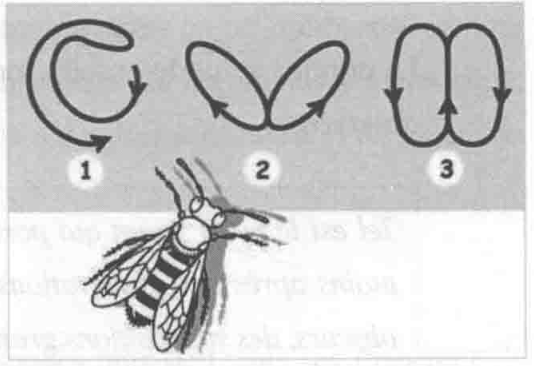
\includegraphics[width=.43\linewidth]{assets/bee_dances_original.png}\end{center}
\origpage{51}{037}
\minititle{1. La danse circulaire}
Avec cette danse, les abeilles décrivent des cercles horizontaux successivement de droite à gauche puis de gauche à droite. Elles signalent par ce moyen la présence de nourriture à une faible distance, à moins de 100 m de la ruche. Avec cette danse, une seule information est transmise : il y a de la nourriture proche.
\minititle{2. La danse en faucille}
Si la source de nourriture se trouve à une distance un peu plus grande (entre 100 m et 6 km de la ruche), l’abeille passe à un second type de danse, la danse en faucille. Elle parcourt désormais deux ellipses allongées et symétriques l’une de l’autre par rapport à un axe. La danse en faucille comporte une information précise sur la direction à suivre : l’angle formé entre son axe de symétrie et la direction verticale est le même que celui entre la direction du soleil et celle vers laquelle il faut voler pour trouver le lieu de butinage. La précision est géométrique, mais la danse en faucille n’indique qu’une distance générale.
\minititle{3. La danse frétillante}
Cette imprécision sur la distance est réglée avec la troisième danse, appelée frétillante car l’abeille y décrit une forme de « 8 » aplati et dont la partie centrale est en ligne droite. L’abeille parcourt cette ligne en faisant frétiller son abdomen. Il existe un lien direct entre la durée du frétillement et la distance à parcourir : plus l’abeille frétille, plus il faudra voler loin. La relation est presque mathématique, proportionnelle : la danseuse frétille pendant 0,8 seconde pour coder 200 mètres, 1,2 seconde pour coder 300 mètres, 1,6 seconde pour coder 400 mètres, etc. Le message transmis ici contient trois données extraites de l’environnement : l’existence d’une source de nourriture, sa distance, sa direction. Contrairement à la première danse, l’existence d’une source de nourriture est implicite dans la danse en faucille et la danse frétillante.
\subsubsection*{2\quad Les premières conclusions}
De prime abord, la communication des abeilles semble partager de nombreux points communs avec le langage humain. Mais elle possède des limitations qui permettent de tracer une frontière nette entre les deux.
\minititle{1. Points communs avec le langage humain}
Les abeilles sont capables de produire (coder) et d’interpréter (décoder) de véritables messages. Elles peuvent enregistrer les données de position et de distance des sources de nourriture, les conserver en mémoire, puis les communiquer à travers l’expression de symboles comportementaux. Il semble également que l’on puisse retrouver chez les abeilles les caractéristiques d’un langage : appartenance à une même espèce, usage d’un même code et existence d’une forme rudimentaire de symbolisme, puisque la forme et la fréquence de la danse transposent visuellement une réalité d’une autre nature. On pourrait rajouter la présence de quelque chose qui ressemble à un système rudimentaire : dans le cas de la danse frétillante, on l’a vu, trois \origcont{52}{038}données de signification sont combinées en un seul message. Nous avons donc bien un système de communication : toutes les abeilles sont capables en dansant d’émettre et de recevoir des signaux compréhensibles par toutes les abeilles de la communauté. Ce système repose en outre sur une convention stable entre le signal (danse) et la réalité à laquelle il réfère (nourriture, distance, direction). Mais c’est ici que la comparaison avec notre langage humain s’arrête.
\minititle{2. Les limites du « langage » animal}
Pour pousser un peu plus loin ses expériences, Karl von Frisch a placé un verre d’eau sucrée au sommet d’un pylône de radiodiffusion au pied duquel se trouvait une ruche. Les abeilles rentrées à la ruche après avoir découvert la source de nourriture n’ont pas réussi à indiquer la direction et la distance aux autres abeilles, qui sont parties dans tous les sens mais n’ont pas trouvé le repas qui pourtant se trouvait juste au dessus de leur tête. La raison ? Leur « langage » ne peut pas exprimer la notion de hauteur car, comme l’exprime joliment Karl Von Frisch, « Les fleurs ne poussent pas les nuages ».\ednote{原文 « Les fleurs ne poussent pas les nuages » 缺介词，应为 « Les fleurs ne poussent pas dans les nuages »。此注只订正句法，不据此独立确证引语的原始出处。}
\subsection{Émile Benveniste : caractéristiques du langage humain}
Secrétaire de Société de Linguistique de Paris de 1959 à 1970, professeur de grammaire comparée au Collège de France 1937 à 1969, le linguiste français d’origine syrienne \textbf{Émile Benveniste} (1902-1976) s’est intéressé aux expériences de Karl Von Frisch. Dans son ouvrage \textit{Problèmes de linguistique générale} (1966 et 1974), en s’appuyant sur les limites du « langage » des abeilles, Benveniste a défini par contraste les caractéristiques du langage humain.
\begin{lecture}{Lecture : \textit{Problèmes de linguistique générale}(extrait)}
Pour nous représenter le fonctionnement d’un « langage » animal, il peut être utile de marquer brièvement en quoi il n’est pas un langage, et comment ces observations sur les abeilles aident à définir, par ressemblance ou par contraste, le langage humain. Les différences sont considérables et elles aident à prendre conscience de ce qui caractérise en propre le langage humain. Celle-ci, d’abord essentielle, que le message des abeilles consiste entièrement dans la danse, sans intervention d’un appareil « vocal », alors qu’il n’y a pas de langage sans voix.\ednote{此句为原引文的历史性主张，不在引文内改写。若作为一般定义，“没有声音就没有语言”排除了手语；本章第 031 页已把手语与口语相提并论。应区分语言系统与发声模态，不能将声音视为语言的必要条件。} D’où, une autre différence, qui est d’ordre physique. N’étant pas vocale mais gestuelle, la communication chez les abeilles s’effectue nécessairement dans des conditions qui permettent une perception visuelle, sous l’éclairage de jour ; elle ne peut avoir lieu dans l’obscurité. Le langage humain ne connaît pas cette limitation. Une différence capitale apparaît aussi dans la situation où la communication a lieu. Le message des abeilles n’appelle aucune réponse de l’entourage, sinon une certaine conduite, qui n’est pas une réponse. Cela signifie que les abeilles ne connaissent pas le dialogue, qui est la condition du langage humain. Nous parlons à d’autres qui parlent, telle est la réalité humaine. Cela révèle un nouveau contraste. Parce qu’il n’y a pas de dialogue pour les abeilles, la communication se réfère seulement à une certaine donnée objective. Il ne peut y avoir de communication relative à une donnée « linguistique » ; déjà parce qu’il n’y a pas de réponse, la réponse étant une réaction linguistique à une manifestation linguistique ; mais aussi en \origcont{53}{039}ce sens que le message d’une abeille ne peut être reproduit par une autre qui n’aurait pas vu elle-même les choses que la première annonce. On n’a pas constaté qu’une abeille aille par exemple porter dans une autre ruche le message qu’elle a reçu dans la sienne, ce qui serait une manière de transmission ou de relais. On voit la différence avec le langage humain, où, dans le dialogue, la référence à l’expérience objective et la réaction à la manifestation linguistique s’entremêlent librement et à l’infini. [...]
\end{lecture}
Pour Benveniste, la conclusion s’impose : le soi-disant « langage » des abeilles n’est pas un langage mais un code de signaux. Voilà la question tranchée.
\subsection{Communication humaine et animale : tableau récapitulatif}
Le tableau ci-dessous récapitule et complète les arguments de Benveniste sur les différences entre la communication humaine et animale.\ednote{仅依本章第 037–038 页，蜜蜂已能传达不在蜂巢现场的食物位置，因此把动物交际一概限定为“此时此地”与本章自己的实例冲突。应区分有限的空间移位能力与人类语言可谈论过去、假设等更广泛的移位能力；不能把“动物没有人类语言的全部特征”改写成“所有动物完全没有其中任一特征”。}
\begin{center}\small\renewcommand{\arraystretch}{1.2}
\begin{tabularx}{\linewidth}{|>{\centering\arraybackslash}p{.21\linewidth}|>{\centering\arraybackslash}X|>{\centering\arraybackslash}X|}
\hline
\textbf{Différences}&\textbf{Communication humaine}&\textbf{Communication animale}\\\hline
Déplacement&Peut évoquer le passé, le futur, l’absent, l’hypothétique et l’impossible&Limitée au présent temporel et spatial : « ici et maintenant »\\\hline
Apprentissage&acquis&inné\\\hline
Unités&divisibles et combinables&indivisibles et non combinables\\\hline
Mutualité&fréquente&rare\\\hline
Mensonges, divagations&fréquents&non\\\hline
Métalangage&oui&non\\\hline
Polysémie&oui&Non (Monosémie)\\\hline
\end{tabularx}
\end{center}
Parmi les éléments présentés dans le tableau ci-dessus, j’attire votre attention sur deux d’entre eux :
\begin{itemize}
\item Le déplacement. Il s’agit de la faculté propre aux humains de pouvoir parler du passé, du futur, d’imaginer, de supposer, d’évoquer, etc. Cette caractéristique constitue l’une des manifestations les plus intéressantes de notre langue. Sans déplacement, pas de création littéraire, pas d’histoire, et pas de sciences, non plus.
\item Le métalangage. Les méta-outils vus plus haut sont des outils utilisés pour faire des outils, le métalangage est le langage utilisé pour parler du langage. Le langage humain est en effet le seul à pouvoir se prendre lui-même comme objet, quand on l’utilise par exemple pour commenter un texte, ou expliquer un mot. Avec la fonction conative rencontrée dans le premier chapitre, la fonction métalinguistique est une des six fonctions du langage.
\end{itemize}
C’est sur ce concept de métalangage que se conclut notre deuxième chapitre introductif. Le texte de Benveniste a été l’occasion d’un premier contact avec la linguistique : dans les 14 chapitres à venir, nous ne la quitterons plus. Nous allons en effet aborder à présent la première grande partie de notre livre, consacrée à la genèse de cette science très jeune qu’est la linguistique.
\origpage{54}{040}
\section*{Exercices}\phantomsection\addcontentsline{toc}{section}{Exercices}\markright{Exercices}
\noindent\textbf{I.\quad Dans sa \textit{Lettre au Marquis de Newcastle} (1646), Descartes oppose le monisme au dualisme, les passions aux pensées, la \textit{phonê} au \textit{logos}, l’inné à l’acquis, le parfait à l’imparfait. Retrouvez ces oppositions dans l’extrait suivant.}
\begin{adjustwidth}{4mm}{4mm}\small
Pour ce qui est de l’entendement ou de la pensée que Montaigne et quelques autres attribuent aux bêtes, je ne puis être de leur avis [...] Il n’y a aucune de nos actions extérieures, qui puisse assurer ceux qui les examinent, que notre corps n’est pas seulement une machine qui se remue de soi-même, mais qu’il y a aussi en lui une âme qui a des pensées, excepté les paroles, ou autres signes faits à propos des sujets qui se présentent, sans se rapporter à aucune passion. Je dis les paroles ou autres signes, parce que les muets se servent de signes en même façon que nous de la voix; et que ces signes soient à propos, pour exclure le parler des perroquets, sans exclure celui des fous, qui ne laisse pas d’être à propos des sujets qui se présentent, bien qu’il ne suive pas la raison; et j’ajoute que ces paroles ou signes ne se doivent rapporter à aucune passion, pour exclure non seulement les cris de joie ou de tristesse, et semblables, mais aussi tout ce qui peut être enseigné par artifice aux animaux; car si on apprend à une pie à dire bonjour à sa maîtresse, lorsqu’elle la voit arriver, ce ne peut être qu’en faisant que la prolation de cette parole devienne le mouvement de quelqu’une de ses passions; à savoir, ce sera un mouvement de l’espérance qu’elle a de manger, si l’on a toujours accoutumé de lui donner quelque friandise, lorsqu’elle l’a dit; et ainsi toutes les choses qu’on fait faire aux chiens, aux chevaux et aux singes, ne sont que des mouvements de leur crainte, de leur espérance, ou de leur joie, en sorte qu’ils les peuvent faire sans aucune pensée. Or il est, ce me semble, fort remarquable que la parole, étant ainsi définie ne convient qu’à l’homme seul. Car, bien que Montaigne et Charron aient dit qu’il y a plus de différences d’homme à homme, que d’homme à bête, il ne s’est toutefois trouvé aucune bête si parfaite, qu’elle ait usé de quelque signe, pour faire entendre à d’autres animaux quelque chose qui n’eût point de rapport à ses passions ; et il n’y a point d’homme si imparfait, qu’il n’en use ; en sorte que ceux qui sont sourds et muets inventent des signes particuliers, par lesquels ils expriment leurs pensées. Ce qui me semble un très fort argument pour prouver que ce qui fait que les bêtes ne parlent point comme nous, est qu’elles n’ont aucune pensée, et non point que les organes leur manquent. Et on ne peut dire qu’elles parlent entre elles, mais que nous ne les entendons pas ; car, comme les chiens et quelques autres animaux nous expriment leurs passions, ils nous exprimeraient aussi bien leurs pensées, s’ils en avaient.
\end{adjustwidth}
\Needspace{13\baselineskip}
\origpage{55}{041}
\noindent\textbf{II.\quad Trouvez à quels animaux correspondent les signaux vocaux suivants :}
\begin{center}\renewcommand{\arraystretch}{1.1}
\begin{tabularx}{.9\linewidth}{XXX}
Barrir&Bramer&Glapir\\
Bêler&Cacarder&Glouglouter\\
Bêler&Cancaner&Grogner\\
Beugler&Caqueter&Hennir\\
Blatérer&Chanter&Hululer\\
Bourdonner&Couiner&Japper\\
Braire&Croasser&Meugler\\
Pépier&Piailler&Rugir\\
\end{tabularx}
\end{center}
\noindent\ednote{底本左列第 2、3 行均印为 « Bêler »，此处保留重复。它可能是重复排印，也可能要求对应不同动物；缺少答案或编者说明，不擅自换入另一个动词。}
\section*{Pour aller plus loin}\phantomsection\addcontentsline{toc}{section}{Pour aller plus loin}\markright{Pour aller plus loin}
\begingroup\small\setlength{\parindent}{-4mm}\leftskip=4mm
BATESON (Gregory). \textit{Communication et société}. Paris, Seuil, 1988.

CONDILLAC (Etienne d.). \textit{Traité des animaux}. Paris, Vrin, 2004.

EKMAN (Paul). \textit{What the Face Reveals}. Oxford University Press, 1989.

FRISCH (Karl V.). \textit{Vie et mœurs des abeilles}. Coll. « Sciences d’aujourd’hui ». Paris, Albin Michel, 1955.

GALLUP (Gordon J.). \textit{Chimpanzees}. Self Recognition, Volume 167, American Association for the Advancement of Science, 1970.\ednote{此处 « Gordon J. » 与本章正文第 026 页的 « Gordon G. Gallup » 不一致；应为 Gordon G. Gallup。}

GOODALL (Jane). \textit{My Life with the Chimpanzees}. Byron Press Visual Publications, 1988.

KAMBOUCHNER (Denis). \textit{Les Méditations métaphysiques de Descartes}. Introduction générale, Première Méditation, PUF, 2005.

PREMACK (David). \textit{Intelligence in ape and man}. London, Erlbaum Associates, 1976.

TOMASELLO (Michael). \textit{Primate Cognition}. Oxford University Press, 1997.
\par\endgroup
\clearpage
\origpage{56}{042}
\section*{Glossaire}\phantomsection\addcontentsline{toc}{section}{Glossaire}\markright{Glossaire}
\gloss{acquis\quad 习得的}{通过学习获得的。}
\gloss{inné\quad 内在的}{事物本身所固有的。\ednote{本章中 inné 与 acquis 对举，表示“先天的／与生俱来的”，而非仅指“内在的”。宜将此词条译作“inné 先天的：与生俱来的，而非通过后天学习获得的”。这是词义订正，不改变正文有关先天与习得的原有论述。}}
\gloss{intentionnalité\quad 意向性，意图性}{对需求对象进行持续关注的意识特点。}
\gloss{métalangage\quad 元语言}{用于分析和描述语言的语言。}
\gloss{polysémie\quad 一词多义}{指一个词有两个或两个以上密切相关的意义。}
\gloss{syntaxe/syntaxique\quad 句法／句法的}{句法研究单词如何组成句子的方式以及掌管句子构成的规则，是语言语法的主要部分。}
